\BgThispage


\section{1322. Шпион}
\textit{Условие задачи:} \par
Спецслужбы обнаружили действующего иностранного агента. Шпиона то есть. Установили наблюдение и выяснили, что каждую
неделю он через Интернет посылает кому-то странные нечитаемые тексты. Чтобы выяснить, к какой информации получил доступ
шпион, требуется расшифровать информацию. Сотрудники спецслужб проникли в квартиру разведчика, изучили шифрующее устройство
и выяснили принцип его работы. На вход устройства подается строка текста $S_1$ = $s_1$$s_2$...$s_N$. Получив ее, устройство
строит все циклические перестановки этой строки, то есть $S_2$ = $s_2$$s_3$...$s_N$$s_1$, ..., $S_N$ = $s_N$$s_1$$s_2$...$s_{N-1}$.
Затем множество строк $S_1$, $S_2$, ..., $S_N$ сортируется лексикографически по возрастанию. И в этом порядке строчки
выписываются в столбец, одна под другой. Получается таблица размером N $\times$ N. В какой-то строке K этой таблицы
находится исходное слово. Номер этой строки вместе с последним столбцом устройство и выдает на выход.\\
Например, если исходное слово $S_1$ = \textit{abracadabra}, то таблица имеет такой вид:
\begin{enumerate}
    \item \textit{aabracadabr} = $S_11$
    \item \textit{abraabracad} = $S_8$
    \item \textit{abracadabra} = $S_1$
    \item \textit{acadabraabr} = $S_4$
    \item \textit{adabraabrac} = $S_6$
    \item \textit{braabracada} = $S_9$
    \item \textit{bracadabraa} = $S_2$
    \item \textit{cadabraabra} = $S_5$
    \item \textit{dabraabraca} = $S_7$
    \item \textit{raabracadab} = $S_10$
    \item \textit{racadabraab} = $S_3$
\end{enumerate}
И результатом работы устройства является число 3 и строка \textit{rdarcaaaabb}.
Это все, что известно про шифрующее устройство. А вот дешифрующего устройства не нашли. Но поскольку заведомо известно,
что декодировать информацию можно (а иначе зачем же ее передавать?), Вам предложили помочь в борьбе с хищениями секретов
и придумать алгоритм для дешифровки сообщений. А заодно и реализовать дешифратор.
\newpage
\textit{Пояснение к примененному алгоритму:} \par
Пусть \textit{M} - матрица всех перестановок, отсортированная лексикографически, \textit{$M_S$} - неотсортированная матрица всех перестановок \textit{F} - первый столбец, \textit{L} - последний, \textit{S} - исходная строка.  \par
\textbf{Теорема 1 (отображение L$\leftrightarrow$F)} Для каждого символа \textit{c}, \textit{i-е} вхождение \textit{c} в \textit{L} соответствует
тому же символу в \textit{S}, что и \textit{i-е} вхождение \textit{c} в \textit{F}, для каждого \textit{i}. \par
\textbf{Доказательство:} Определим правый контекст символа \textit{$F_i$} как \textit{n-1} оставшихся столбцов матрицы \textit{M}.
В \textit{F} все вхождения \textit{c} находятся вместе в одном интервале, и они упорядочены по их правому контексту.
В \textit{L} вхождения \textit{c} могут быть разбросаны по \textit{L}, но они также упорядочены по их правому контексту,
поскольку \textit{$M_S$} состоит из циклических вращений. Поскольку они отсортированы в соответствии с одной и той же строкой,
они расположены в одном и том же порядке. Вот рисунок, иллюстрирующий приведенное выше доказательство:
\begin{figure}[H]
    \centering
    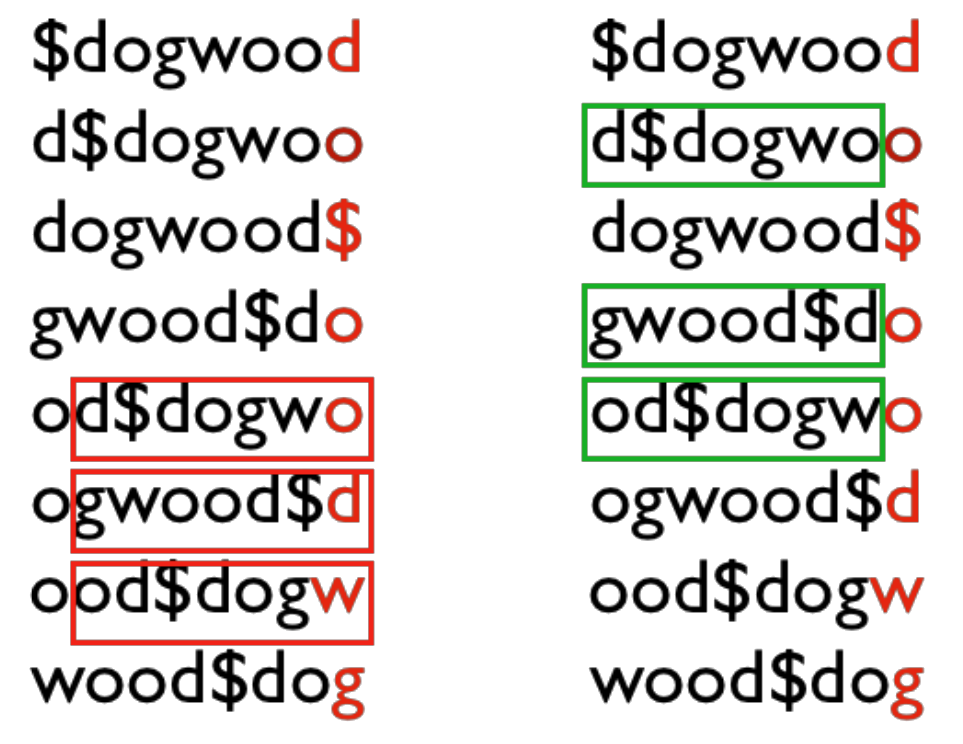
\includegraphics[scale=0.2]{img/proof}
\end{figure}
\BgThispage
\newpage
\begin{wrapfigure}{r}{0.25\textwidth} %this figure will be at the right
    \centering
    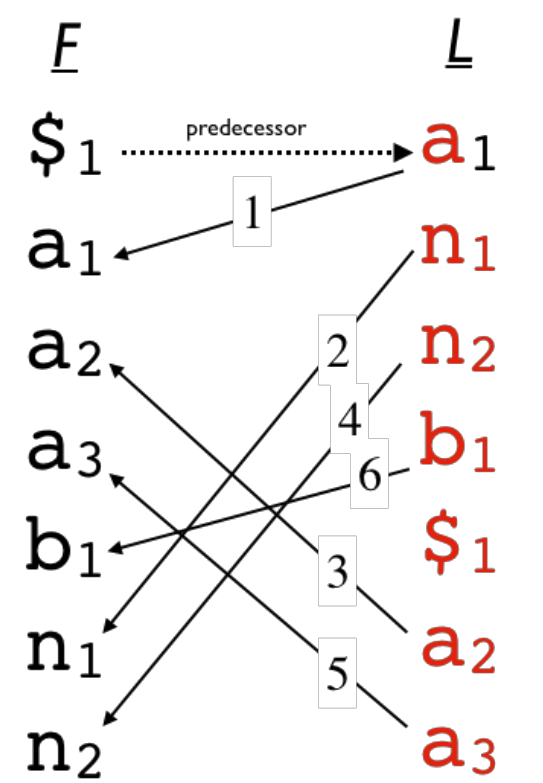
\includegraphics[width=0.25\textwidth]{img/example2}
\end{wrapfigure}
Свойство L$\leftrightarrow$F позволяет нам инвертировать шифрование напрямую. Мы восстанавливаем \textit{S}, начиная с конца \textit{S}.
\textit{S} заканчивается на \$, который является первым символом \textit{F}. Какой символ идет в $S$ перед \$? Первый
символ стобца \textit{L}. Итак, теперь мы знаем, что \textit{S} заканчивается на $L_0$\$. Это общий случай: пары
($L_i$ , $F_i$) дают отношения предшествования. То есть, $F_i$ это символ, непосредственно предшествующий $L_i$ в $S$.
Это следует (опять же) из того факта, что мы имеем дело с циклическими вращениями. Продолжим наш пример: Мы знаем,
что строка заканчивается на $L_0$$F_0$, и теперь мы хотим найти предшественника $L_0$. Для этого нам нужно найти правильное
вхождение $L_0$ в $F$. Вот где мы используем свойство отображения L$\leftrightarrow$F: Если $L_0$ является \textit{i-м} вхождением
символа $L_0$ в $L$, тогда соответствующий символ является \textit{i-м} вхождением символа $L_0$ в $F$.\\
\\
\vspace{0.7cm}
\\
Собственно, так и реализован мой алгоритм: я составляю соответствия между $L_i$$F_i$, сопоставляя \textit{i-му} вхождению $c$ в $L$
\textit{i-е} вхождение $c$ в $F$. Так как ограничение по времени не позволяет обойти $L$ и $F$ "в тупую", я использую бинарный поиск
по $F$, так как $F$ отсортирована - нахожу любое вхождение $c$ в $F$, перемещаюсь к первому вхождению $c$, а потом отступаю на
столько символов, сколько вхождений уже было найдено. Таким образом, формируется массив $N$, где в каждом $N_i$ записан
индекс $j$, а $i$,$j$ такие, что $F_i$ = $L_j$ = $c$ (дублирование $c$ учтено и описано выше). По известному номеру строки,
содержащей $S$, я нахожу начало $S$, а дальше вывожу всю строку: для каждого $i$, $F_i$ - буква, очерёдность которой в $S$ совпадает с
очерёдностью вызова $i$, а $N_i$ - новый $i$ для следующего шага.\par
Сложность алгоритма: |O($Nln(N)$) - сортировка F| + |O($Nln(N)$) - бинпоиск N символов| + |операции с unordered\_map O(1)| $\approx$ \underline{O($Nln(N)$)}
\BgThispage
\newpage
\textit{Код:}
\small
\begin{center}
    \begin{verbatim}
    uint32_t N;
    std::string line;
    std::cin >> N >> line;
    std::string sorted_line = line;
    std::sort(sorted_line.begin(), sorted_line.end());
    std::vector<int> list(line.length());
    std::unordered_map<char, int> count_literals;
    for (int i = 0; i < line.length(); ++i) {
        int L = 0;
        int R = sorted_line.length() - 1;
        int M;
        while (R - L > 1) {
            M = (R + L) / 2;
            if (sorted_line[M] > line[i]) R = M;
            if (sorted_line[M] < line[i]) L = M;
            if (sorted_line[M] == line[i]) break;
        }
        if (sorted_line[M] != line[i]) {
            if (sorted_line[M-1] == line[i]) M--;
            if (sorted_line[M+1] == line[i]) M++;
        }
        while (M > 0 && sorted_line[M] == sorted_line[M - 1]) {
            M--;
        }
        int shift = 0;
        if (count_literals.find(sorted_line[M]) != count_literals.end()) {
            shift = count_literals.at(sorted_line[M]);
            count_literals.at(sorted_line[M])++;
        } else {
            count_literals.emplace(sorted_line[M], 1);
        }
        list[M + shift] = i;
    }
    uint32_t x = N - 1;
    for (int i = 0; i < list.size(); ++i) {
        std::cout << sorted_line[x];
        x = list[x];
    }
    return 0;
    \end{verbatim}
\end{center}
\normalsize
\BgThispage
\newpage


\section{1604. В Стране Дураков}
\textit{Условие задачи:} \par
Главный бульдог-полицейский Страны Дураков решил ввести ограничение скоростного режима на автомобильной трассе, ведущей
от Поля Чудес к пруду Черепахи Тортиллы. Для этого он заказал у Папы Карло n знаков ограничения скорости. Папа Карло
слабо разбирался в дорожном движении и поэтому изготовил знаки с разными ограничениями на скорость: 49 км/ч, 34 км/ч, 42 км/ч, и т.д.
Всего получилось k различных ограничений: n1 знаков с одним ограничением, n2 знаков со вторым ограничением, и т.д. ($n_1$ + … + $n_k$ = $n$)
Бульдог-полицейский ничуть не расстроился, получив такие знаки, напротив, он решил извлечь из этого экономическую выгоду.
Дело в том, что по Правилам дорожного движения Страны Дураков ограничение на скорость действует вплоть до следующего знака.
Если на знаке написано число 60, это означает, что участок от данного знака до следующего нужно проехать ровно со скоростью
60 километров в час — не больше и не меньше. Бульдог распорядился расставить знаки так, чтобы обогатившимся на Поле Чудес
автолюбителям во время своего движения по трассе приходилось как можно больше раз менять скорость. Для этого нужно расставить
имеющиеся знаки в правильном порядке. Если Вы поможете бульдогу это сделать, то он готов будет поделиться с Вами частью своих доходов.\\
\textit{Пояснение к примененному алгоритму:} \par
Мой алгоритм выбирает на каждом шаге существующий максимум по количеству знаков одного вида, отличный от предыдущего (другой знак),
и ставит знак этого вида.\\
\textbf{Доказательство:} \par
Очевидно, что максимальное количество смен скоростей в последовательности ограничено сверху $n$.
Пусть таким алгоритмом количество смен скоростей по итогу получилось меньше, чем n. Значит, в полученной
строке идут неодинаковые пары, а в конце плато (выбираем максимумы, пока можем чередовать, а после подряд ставим оставшиеся знаки одного вида):
$n_0$,$n_i$ , ... , $n_j$,$n_0$, ... , $n_0$.
Рассмотрим другую возможность расположить знаки в последовательности так, чтобы количество смен скоростей было максимально,
и предположим, что количество смен знаков в таком случае будет больше. Тогда возьмём эту последовательность, и
будем перемещать все $n_i$, соседствующие друг с другом, в конец последовательности так, чтобы плато было только в конце.
Очевидно, что оно будет одно, так как знаки из двух наборов, идущих подряд, мы можем просто чередовать, пока не закончится один из них.
Заметим, что в таком случае мы получим нашу исходную последовательность. Значит, количество смен знаков в рассматриваемой последовательности
такое же, как в исходной. Противоречие.
\BgThispage
\newpage
\textit{Код:}
\small
\begin{center}
    \begin{verbatim}
void findMaxEl(std::vector<size_t> *vec, size_t *iter) {
    size_t max = (*vec)[*iter];
    for (size_t i = (*iter)+1; i < (*vec).size(); ++i) {
        if ((*vec)[i] > max) {
            max = (*vec)[i];
            *iter = i;
        }
    }
}

void findPredMaxEl(std::vector<size_t> *vec, size_t *jiter, size_t *iter) {
    size_t max = 0;
    for (size_t i = (*jiter)+1; i < (*vec).size(); ++i) {
        if (i!=(*iter) && (*vec)[i] > max) {
            max = (*vec)[i];
            *jiter = i;
        }
    }
}

int main() {
    size_t k;
    std::cin >> k;
    std::vector<size_t> n(k);
    for (int i = 0; i < k; ++i) {
        size_t m;
        std::cin >> m;
        n[i] = m;
    }
    size_t iter = 0;
    findMaxEl(&n,&iter);
    while (n[iter]>0) {
        std::cout << iter+1 << " ";
        n[iter]--;
        size_t jiter = 0;
        findPredMaxEl(&n,&jiter,&iter);
        if (n[jiter] > 0) {
            std::cout << jiter +1 << " ";
            n[jiter]--;
        }
        iter = 0;
        findMaxEl(&n,&iter);
    }
    return 0;
}
    \end{verbatim}
\end{center}
\normalsize
\BgThispage
\newpage
